\subsubsection{Static analysers}
\label{sec:static-analysers}
We introduce static analysis tools to our project's build setup to help in tracking functional, non-functional and stylistic defects in the code. Three of the tools (PMD, JDepend and FindBugs) target bugs in Java code. However, no defects were detected by any of the tools.
\par 
Checkstyle on the other hand, is used to evaluate the code writing style of the application - and is very much needed for this project. The tool flagged around 2000 code style errors when run, most of which related to whitespace misuse, variable name oddities... The tool can be configured to suite the code conventions set out for the project and can be made to ignore certain warnings. 
\par
The tools can all be made to run through the gradle task "check". 

\begin{figure}[H]
\centering
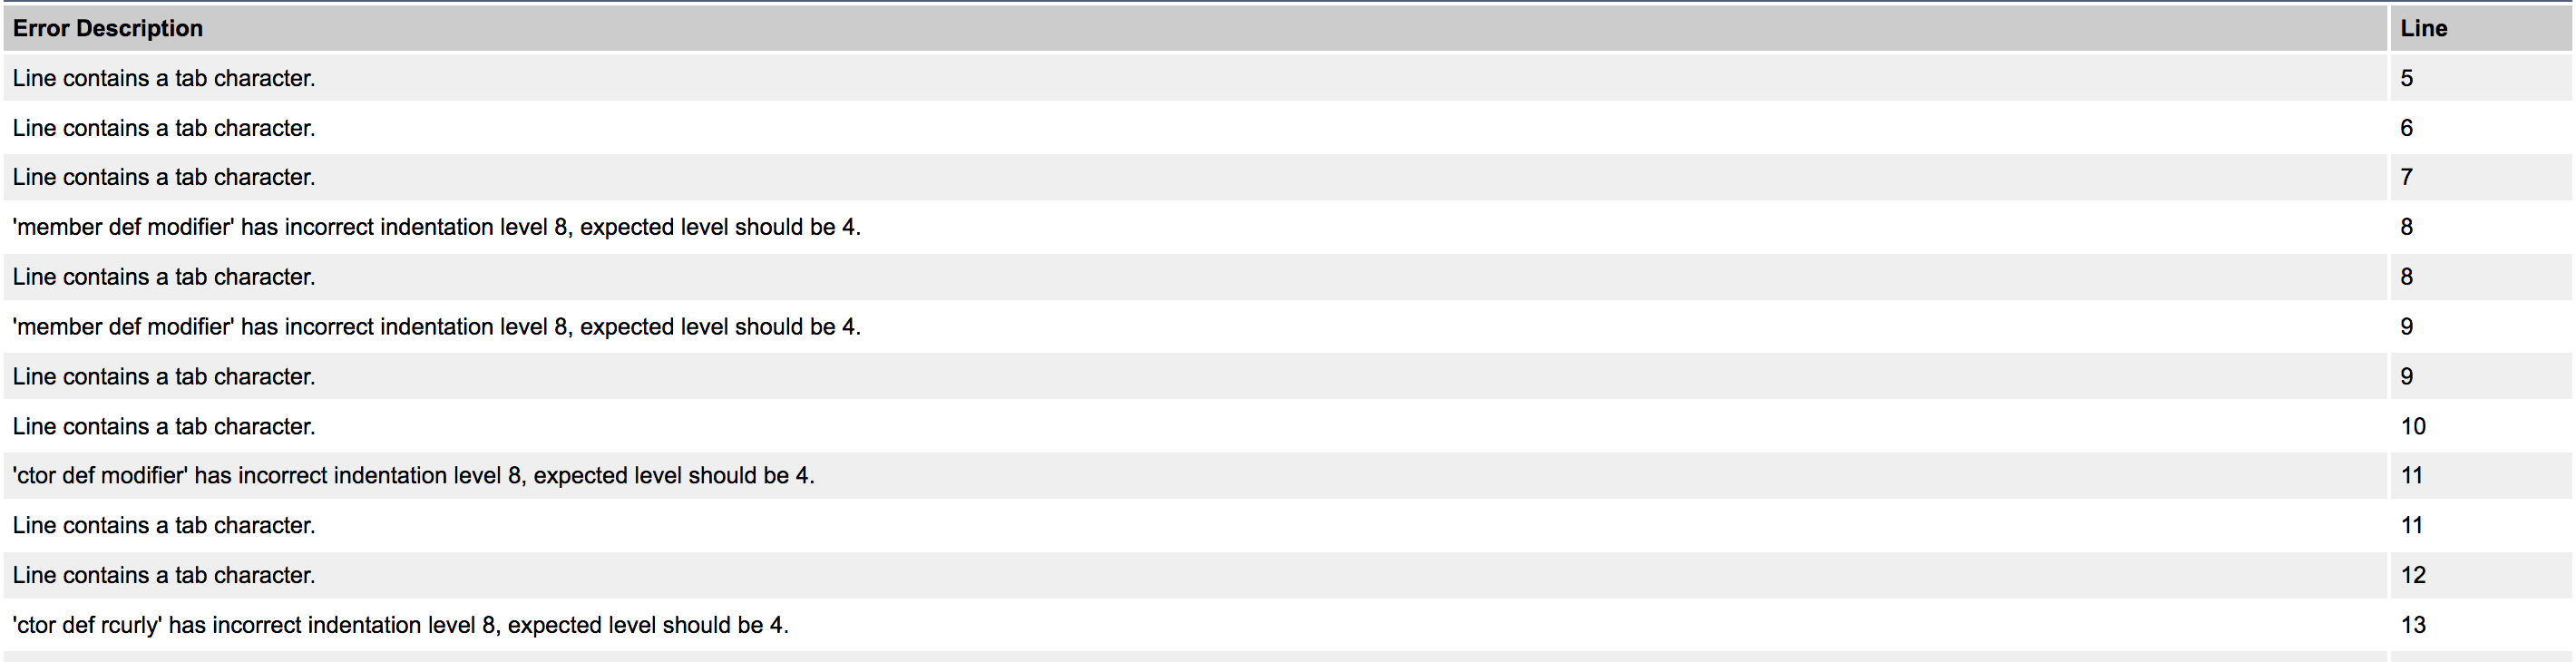
\includegraphics[width=\textwidth]{res/checkstyle.png}
\caption{Checkstyle output}
\end{figure}